
%%% Local Variables:
%%% mode: latex
%%% End:



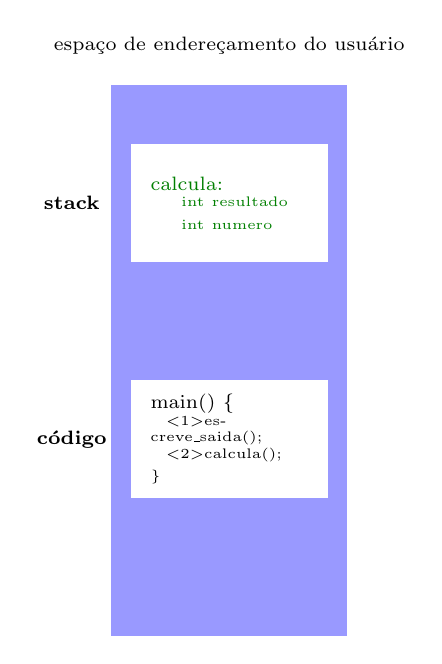
\begin{tikzpicture}
  \tikzset{every node/.style={font=\scriptsize},
    userspace/.style={color=blue,fill=blue!40, minimum width=3cm,
      minimum height=7cm,text width=2.5cm,anchor=north},
    resource/.style={text width=2cm, minimum width=2.5cm,
      minimum height=1.5cm,fill=white}}
  \colorlet{calcula}{green!50!black}
  \colorlet{io}{blue!50!black}
  
  \node[userspace] (useraddress) {};
  \node[] (label) [above of=useraddress,yshift=3cm] {espaço de endereçamento do usuário};

  \node<1>[color=blue,resource,align=left] (routine) [below of=label,yshift=-1cm] {escreve\_saida: \\ \tiny \hspace{.3cm} FILE $*$arquivo\\\hspace{.3cm} char $*$conteudo};
  \node<2>[calcula,resource,align=left] (routine) [below of=label,yshift=-1cm] {calcula: \\ \tiny \hspace{.3cm} int resultado\\\hspace{.3cm} int numero};
  \node [left of=routine,xshift=-1cm] {\bf stack};
  \node[resource,align=left] (code) [below of=routine,yshift=-2cm] 
  {main() $\{$\\\hspace{.2cm}{\tiny \alert<1>{escreve\_saida();} \\\hspace{.2cm}\alert<2>{calcula();}\\$\}$}};
  \node [left of=code,xshift=-1cm] {\bf código};
\end{tikzpicture}
